\documentclass[12pt,oneside]{book}
% pouzite balicky
\usepackage[latin2]{inputenc}
\usepackage{amsmath}
\usepackage[czech]{babel}

\RequirePackage{ifpdf}
\ifpdf
  \RequirePackage[pdftex]{graphicx}
  \RequirePackage[pdftex]{color}
  \RequirePackage{ps4pdf}
\else
  \RequirePackage[dvips]{graphicx}
  \RequirePackage[dvips]{color}
  \RequirePackage{pstricks}
\fi

\usepackage{pst-all}

\usepackage{pslatex}
\usepackage{url} 
\usepackage{hyperref} 

\usepackage{listings}
\usepackage{array}
\usepackage{multirow}
\usepackage{comment}
\usepackage{lscape}
\usepackage{rotating}

%\usepackage{nopageno}
\usepackage{geometry}
\geometry{paperwidth=8.26in,paperheight=11.69in,
          left=4cm,right=3cm,
          top=3.5cm,bottom=3.5cm}

\usepackage{float}
\floatstyle{ruled}

\newfloat{algorithm}{thp}{loa}
\floatname{algorithm}{Algoritmus}

\newtheorem{theorem}{V�ta}

\newtheorem{definition}{Definice}

\newcommand{\etalchar}[1]{$^{#1}$}
\sloppy
%%%%%%%%%%%%%%%%%%%%%%%%%%%%%%%%%%%%%%%%%%%%%%%%
\title{This is my first document}
\author{Vaclav Klecanda}
\date{31.1.2009}
\begin{document}

\pagestyle{empty}

\include{diplomka_titlepage}
\pagestyle{empty}


\vspace*{1em}




%%%%%%%%%%%%%%%%%%%%%%%%%%%%%%%%%%%%%%%%%%%%%%%%%%%%%%%%%%%%%%%%%%%%%%%%%%%%%%%%
%   Pod�kov�n�

\begin{figure}[t]

\par
%D�kuji RNDr. Pelik�novi za cenn� rady a p�ipom�nky k~t�to pr�ci. MUDr. Hor�kovi za poskytnut� l�ka�sk�ch znalost� a dat. Mgr. Mar��lkovi za pomoc a podporu.

\end{figure}

%\pagebreak




%%%%%%%%%%%%%%%%%%%%%%%%%%%%%%%%%%%%%%%%%%%%%%%%%%%%%%%%%%%%%%%%%%%%%%%%%%%%%%%%
%   Prohl��en�

\vspace*{1em}

\flushbottom

\begin{figure}[b]

\par
%Prohla�uji, �e jsem svou diplomovou pr�ci napsal(a) samostatn� a v�hradn� s~pou�it�m citovan�ch pramen�. Souhlas�m se zap�j�ov�n�m pr�ce.

\vspace{2em}

\begin{tabular*}{1.0\textwidth}[b]{@{\extracolsep{\fill}} l r }
%V~Praze dne 20. Dubna 2007 & V�clav Kraj��ek\\
                           %& vlastnoru�n� podpis
\end{tabular*}

\vspace*{2em}

\end{figure}

\raggedbottom

%%%%%%%%%%%%%%%%%%%%%%%%%%%%%%%%%%%%%%%%%%%%%%%%%%%%%%%%%%%%%%%%%%%%%%%%%%%%%%%%
%   KONEC Podekov�n�
 

\pagestyle{empty}
%--------------------------------------------------------
%-------------             OBSAH            -------------
%--------------------------------------------------------
\tableofcontents

\pagebreak

%--------------------------------------------------------
%-------------       SEZNAM OBRAZKU         -------------
%--------------------------------------------------------
\listoffigures

\pagebreak

%--------------------------------------------------------
%-------------       SEZNAM TABULEK         -------------
%--------------------------------------------------------
\listoftables

%\listof{algorithm}{Seznam algoritmu}

\pagebreak

%--------------------------------------------------------
%-------------           ABSTRAKT           -------------
%--------------------------------------------------------

\section*{submission}
Study available literature and technical documentation about programming on IBM Cell BE architecture. As well as interfaces, development environments and tools for creating programs for CellBE and its particular implementation Play Station 3, IBM system simulator, Cell Blade. Find out its potential and abilities for parallel processing. Learn about design patterns.

Try some algorithm (registration, segmentation) aimed to medical data processing (CT, MR, X-ray images) where huge data sizes are processed and where results has to be get relativelly fast because diagnosis are made for lasg number of patients. It suitable to do comparation study between common PC architecture and CellBE aimed to speed, precision, code complexity and ways of algorithms design itselfs. 

\pagebreak

%vkladani headeru
\pagestyle{headings}

\chapter{CellBE platform}

This chapter will introduce CellBE (Cell Broadband Engine) itself, its specifics. Introduce to my experience with the platform will then follow.

\section{About the processor}

CellBE processor is representative of new generation of IBM's CellBE platform family made by collaboration of IBM, Sony, and Toshiba. CellBE is an asymmetric, high-performance multi-core processor that combines eight synergistic processing elements (SPEs) and a Power Processing Element (PPE), which is a general-purpose IBM Power PC\textregistered core. Each SPE has a 4-way SIMD engine, a high-speed local store and a direct memory access (DMA) engine. The 4-way SIMD unit of each SPE can perform a floating or integer operation on four data elements at every clock tick. Unlike conventional microprocessors, each SPE does not have a hardware cache to manage its small on-chip local store. All the elements are connected through high speed bus (EIB - Element Interconnect Bus). Therefore, this architecture can be viewed as a distributed memory multiprocessor with a very small local memory (local store), under software control, attached to a larger (central) shared memory through DMA engine that manages transfering data from central memory to local store and vice versa.

CellBE achieves a significant performance per Watt and performance per chip area advantage over conventional high-performance processors, and is significantly more flexible and programmable than single-function and other optimized processors such as graphics processors, or conventional digital signal processors. While a conventional microprocessor may deliver about 20+GFlops of single-precision (32b) floating-point performance, Cell delivers 200+ GFlops (in ideal conditions) at comparable power.

A number of signal processing and media applications have been implemented on Cell with excellent results. Advanced visualization such as ray-casting, ray-tracing, and volume rendering. Streaming applications such as media encoders and decoders and streaming encryption and decryption standards have also been demonstrated to perform about an order of magnitude better on Cell than on conventional PC.

TODO obrazek Cellu
\begin{figure}
    \centering
    \includegraphics[height=7.9cm]{medatlas}
    \caption[CellBE processor layout]{Anatomick� atlas - horn� ��st b�icha zep�edu.
      Jsou zde dob�e vid�t ledviny (zelen�).
      Prav� je ��ste�n� p�ekryt� dvan�ctern�kem.
      Slezina (�erven�) le�� vlevo zhruba v~�rovni ledvin a j�tra (mod�e) le�� vpravo vep�edu o~n�co v��e.
      Na obr�zku je vid�t jen jejich ��st.}
    \label{fg:processorLayout}
\end{figure}

\subsection{PPE - PowerPC\textregistered Processing Element}
PPE is derived from IBM Power PC\textregistered core. Has 512kB L2 cache in die. It supports the Power Architecture ISA, inherits the memory translation, protection, and SMP coherence model of mainstream 64-bit Power processors. CBEA also supports virtualization (logical partitioning), large pages, and other recent innovations in the Power architecture. Programming for the PPE is the same as for conventional processors.

\subsection{SPU - Synergistic Processing Element}
SPE is an autonomous processor (sometimes called accellerator) targeted for computational intensive applications. It supports a SIMD-RISC instruction set. Has 128 (128-bit long) unified registers to store all types of data (in contrast from traditional RISCs where registers are devided according data types). One of CellBE programming aspects is converting the code that it uses the SIMD instructions. This process is calleed "SIMDation".

SPE stores its program and data in its associated local storage memory as private memory. DMA transactions are used to tranfer data from/to central memory as well as between two local stores. We say that data is "DMAed" from source to destination. DMA commands can be issued in many ways. Synchronous, asynchronous, in scatter-gaether manner through DMA lists. This memory management is another big part of programming for CellBE.

Programming for SPE has some differencies over programming for conventional processor. You have always to count with the fact you have only 256kB for your program and data. Data is 

This processor is embeded in Sony Playstation 3 game console as well as IBM Blade servers where two or more such processors (as building blocks) connected by high speed bus creates powerfull and modular machine. I have PlayStation3 machine available for my work.

\section{My journey into CellBE platform}
When I started this work I was Windows\textregistered user. Because the developmnet environment (SDK) for CellBE is purely in Linux I had to learn it. I had have already gone through some basic courses so i knew some basic commands. But it is far insufficient when you want to use all the tools for CellBE development. There are some bugs and parts that are not fully finished. Without some kind of deeper knowledge of the system you will have so much troubles as I had. So that's why one of the biggest advice is to become advanced Linux (especially Fedora) user.

The process of advancing my Linux experience went hand in hand with exploration of CellBE platform and the environment. I gradually went through variety of errors and bugs. And I gained more and more experince by their solutions. The process takes quite long time and meanwhile new version of SDK (3.1) had appeard. I wanted to use and describe the latest tools. So I had to begin from scrath because new version brought new obstacles as well.

The new version was declared to be compatible with new version of Fedora (9 - Sulphur) that had been released few months before the new version of SDK. Previous version of SDK (3.0) was for Fedora 7 Warewolf. I tried all possible combinations of Fedoras and SDKs to find out if they are compatible with each other. Only result from that was finding that the are not and lots of days spent on it. Even if I tried Fedora 10 Cambridge that was released as the latest there was some issues. The SDK is huge package of software dependent on lots of third party libraries and solutions that is trated differently within particular distributions and even versions of same distribution. So the next advice is not to combine versions (system, SDK nor particular libraries that the SDK components are dependent on - use repository ones, see Tools installation TODO). There was although some efforts to get it run on another distributions than Fedora. But i thing the time spent is not worth the result.

Finally I installed declared by IBM as working combination consisting of Fedora 9 Sulphur and SDK 3.1 and decided working on it. Altough I have run into some bugs and errors. The process of installation is described in Appendix A. Installation of Fedora is omited. For details see official site http://fedoraproject.org/.

\chapter {Cell/B.E. programming}
\par
Cell/B.E. platform development tools will be described in this chapter.
Our experience with the tools will be mentioned as well.
Then particular SDK content and tools will be listed.
Parallel systems and models will be mentioned later on as well as the relationship to Cell/B.E. development along with a few design patterns.
At the end core configurations and their advantages and disadvantages will be listed finishing with few practical approaches to Cell/B.E. porting process.

\section{Cell/B.E. platform development}
\par
IBM delivers SDK for development of programs for the Cell/B.E. programming.
It made for Linux platform, in the concrete for Fedora or Red Hat distribution.
It comes in two flavors.
The first is the official non free SDK which has all the features needed for development for the Cell/B.E. even for hybrid systems.
The purchaser has also a support team ready to help.
Next is the free one that is open to wide public and everybody can download it and start developing.
The free one does not have full support for hybrid systems nor for development in other languages than C/C++.
Wee have used the free one since we have developed only in C/C++ and for clean Cell/B.E. processor.

\par
Because the SDK is for Linux operation system its user has to have already deeper knowledge about this system.
There are a few bugs and parts that are not fully finished (see Appendix \ref{toolsSetup}) and without this deeper system knowledge is practically impossible to react on unexpected behavior during installation or development phase.

\par
We have begun with SDK version 3.0 and Fedora version 8 which were the current version of needed tools.
We have faced number obstacles and before we were able to overcome them new version of SDK (3.1) appeared.
Because we wanted to use and describe the latest tools we had to begin from scratch because new version brought new obstacles as well.

\par
The new version was declared to be compatible with a new version of Fedora, 9 - Sulphur, that had been released at almost same as the new version of SDK.
The previous version of SDK (3.0) was for Fedora 7 Werewolf.
We have tried all possible combinations of Fedora distributions and SDK packages to find out if they are compatible with each other.
Only result from that was finding that the are not.
We have spent number of days on this discovery.
The SDK is huge package of software dependent on lots of third party libraries and solutions.
They are treated differently within particular distributions and sometimes even versions of the same distribution.
So the result is not to combine system versions nor SDK versions nor particular libraries that the SDK components are dependent on.
Repository versions should be used, see Appendix \ref{toolsSetup}.

\par
Although there are too much of troubles when different version are combined, few efforts to get the SDK run on another distributions than Fedora were made.
But we think the time spent on this goal is not worth the result.

\par
Finally we installed Fedora 9 Sulphur and SDK 3.1.
This combination is declared by IBM as tested.
Altough we have run into few bugs and errors.
The process of installation is described in the Appendix \ref{toolsSetup}.

\section {SDK content}

Cell/B.E. SDK is divided into variety of components.
Each component is contained in one or more rpm package for easy intallation purposes.
Here is list of most important available components:
\begin{enumerate}
  \item {Tool chain}
  \par
  Set of tools such as compilers, linkers etc. necessary for actual code generation.
There are two tool chains.
One is for PPU and the other for SPU.

  \item {Libraries}
  \par
  IBM provides with the SDK several useful libraries for mathematical purposes e.g. linear algebra, FFT, Monte Carlo.
Another libraries set is for cryptography or run-time management.
Code of these libraries is debugged, highly optimized for running on SPEs and SIMDized.

  \item {Full system simulator}
  \par
  Program that can simulate the Cell/B.E. processor on other hardware platforms.
It is used mostly in profiling stage because simulator can simulate actual computation of a code in cycle precision.
It can be of course used when programmer has an actual Cell/B.E. hardware available, but simulation is incredibly slow.

  \item {IDE}
  \par
  IDE is in fact verstion 3.2 of Eclipse with integration of debugging, profiling, Cell/B.E. machine management and other features that makes development for the Cell/B.E. easier and more comfortable.
\end{enumerate}


\section{Parallel systems \& Cell/B.E.}

Parallelism depends also on type of system where the program will be run.
There are two basic kind of parallel systems:
\begin{enumerate}
\item {shared-memory system}
\par
Is multi-processor system with one shared memory which all processor can see.
Processors has to synchronize access to the memory otherwise race conditions will rise.

\item {distributed-memory system}
\par
Is system where each processor has its own private memory.
There is no need for synchronization.
\end{enumerate}

In context of parallel systems, Cell/B.E. is a kind of hybrid system.
SPEs matches the distributed-memory system due to private local stores while PPE is shared-memory system.
Sometimes is Cell/B.E. called heterogeneous multi-core, with distributed memory.
Because Cell/B.E. processors can be gathered into bigger units such as blade server, with two Cell/B.E. chips they can be viewed as either 16 + 2 cores in SMP mode or two non-uniform memory access machines connected together.
Programmer has then to decide which view of the Cell/B.E. processor is better for the solved problem.

\par
Because of separation of address spaces programming of SPE is very similar to client/server application design.
Roles depends on how the work is started.
In case PPU initiate the transfers, the PPU is a client and SPE is a server because SPE receive some data for computation.
Another possibility is that SPE grabs the data from the central memory.
In this case, SPE is a client of central memory.
This case is preferred because the PPE is only one and would not be able to manage all the SPU.

\section{Cell/B.E. programming models}

\par
Implementation of parallel algorithms rely on parallel programming model.
That is a set of software technologies such as programming languages extension, special compilers, libraries through that actual parallelism is achieved.
Programming model is programmer's point of view to the hardware.
So another decision that programmer has to make is to choose a programming model or mixture of them that will best fit for the solved problem.

\par
For Cell/B.E. there is variety of parallel programming models.
Models differ from each other in view of the hardware and thus how many actions are performed implicitly by the model.
The actions can be e.g. task distribution management, data distribution management or synchronization.
The most abstract ones can perform many actions implicitly.
Their advantage is ease of implementation but at cost there can be no performance tuning done.
Differently act the most concrete models that see the Cell/B.E. processor with all the low level details.
Their advantage is performance tuning that can be performed in all the application parts but at cost of more development.

\par
There are several models that are determined only for the Cell/B.E. platform and are contained in SDK.
While there are other models such as MPI, OpenMP that can be used as well but they would expose only PPE.
These will not be further described.

List of the programming models (frameworks) follows in order from most concrete to most abstract:
\begin{enumerate}
\item {libspe2}
\par
This library provides the most low level functionality.
Offer SPE context creating, running, scheduling or deleting.
DMA primitives for data transfer, mailboxes, signal, events, and synchronization functions for PPE to SPE and SPE to SPE dialogs are also provided by this library.
More information can be found in \cite{performanceToolRef} within "SPE Runtime Management Library" document.

\item {Data Communication and Synchronization - DaCS}
\par
Defines program entity for PPE or SPE.
These are HE (Host Element program) for PPE and AE (Accelerator Element program) for SPE.
It provides services for that programs.
The services are e.g. resource and process management, where an HE manipulates its AEs or group management, for defining groups in which synchronization events like barriers can happen or message passing by using send and receive primitives.
More information can be found in \cite{performanceToolRef} within "DACS Programmer's Guide and API Reference" document.

\item {Accelerated Library Framework - ALF}
\par
ALF defines ALF-task as another entity that perform computationally intensive parts of a program.
The idea is to have the host program split the work into multiple independent pieces which are called work blocks.
They are described by a computational kernel, the input and the output data.
Programming with ALF is divided into two side.
The host and the accelerator one.
On the accelerator side, the programmer only has to code the computational kernel, unwrap the input data, and pack the output data when the kernel finishes.
The ALF offer clear separation between host accelerator sides of program parts.
Providing the following services: work blocks queue management, load balancing between accelerators, transparent DMA transfers etc.
More information can be found in \cite{performanceToolRef} within "ALF Programmer's Guide and API Reference" document.

\end{enumerate}

Choosing a framework is important decision of writing Cell/B.E. application.
It should be considered enough.

\subsection {Cell/B.E. parallelism levels}

The Cell/B.E. processor offers many opportunities for parallel processing.
That is because it is composed of heterogeneous elements, SPE and PPE and possibility of particular composition of more processors into more complex systems.
 Levels are:
\begin{enumerate}
\item server level
\par
Parallelism on this level means task distribution among multiple servers like within a server farm.
This is possible in a hybrid environment at the cluster level using MPI or some other grid computing middle-ware.

\item Cell/B.E. chips level
\par
On this level tasks can be divided among multiple Cell/B.E. processors.
This is possible if there are more such processors in one machine.
This is in e.g. blade server with two Cell/B.E. chips.
ALF or DaCS for hybrid can be used for task distribution.

\item SPE level
\par
This parallelism level allow to distribute tasks among particular SPEs.
Libspe, ALF, DaCS can be used to perform the distribution.

\item SIMD instruction level
\par
This level can increase the speed the most.
Paralelism is achieved on instruction level that means more data are processed at a time by single instruction.
Language intrinsics are used for this purpose.
This will be explained later in part devoted to "SIMDation".
\end{enumerate}

\subsection{Computation configurations}

\par
Because of heterogeneous nature of Cell/B.E. there are few computation configurations that can be used.
Each of them differs in usage of SPEs and has its own pros and cons:
\begin{enumerate}
\item Streaming configuration
\par
All SPE serves as a stream processor (see figure \ref{fg:streamingModel}).
They run exactly the same code expecting the same type of data and producing also the same of data type.
This configuration is well suited for streaming application for example filters where there is still the same type of data on input.

\begin{figure}
    \centering
    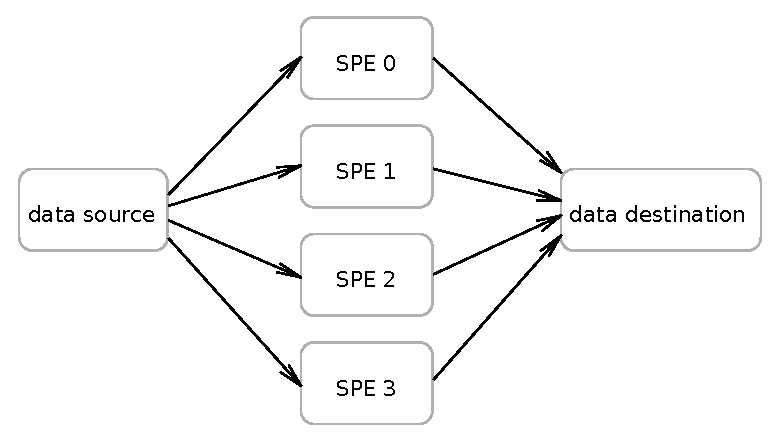
\includegraphics[width=0.9\textwidth]{data/streamingModel}
    \caption[Streaming SPE configuration]{All SPE run the same code creating farm of processor that process same type of data.}
    \label{fg:streamingModel}
\end{figure}

\item Pipeline configuration
\par
SPE server as stages of a pipeline (see figure \ref{fg:pipelineModel}).
Data are passed through from one to other of the SPEs.
The SPE to SPE transfer are faster than SPE to PPE so this can be benefit.

\begin{figure}
    \centering
    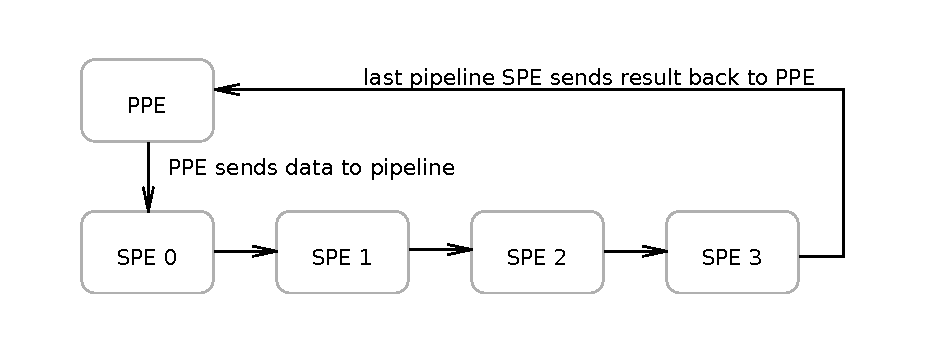
\includegraphics[width=0.9\textwidth]{data/pipelineModel}
    \caption[Pipeline SPE configuration]{SPE creates a pipeline. Each SPE represent one stage of that pipeline. Data are transferred only via SPE to SPE DMA transfers benefiting the speed of bus.}
    \label{fg:pipelineModel}
\end{figure}

\item PPE centric
\par
This configuration is common approach with the Cell/B.E.
Program runs on PPE (see figure \ref{fg:PPUCentricModel}) and only selected, highly demanding computational kernels (hotspots) are offloaded to SPEs.
This method is the easiest from a program development perspective because it limits the scope of source code changes and does not require much re-engineering at the application logic level.
One disadvantage is dynamic changes of SPE contexts that is quite expensive operation.

\begin{figure}
    \centering
    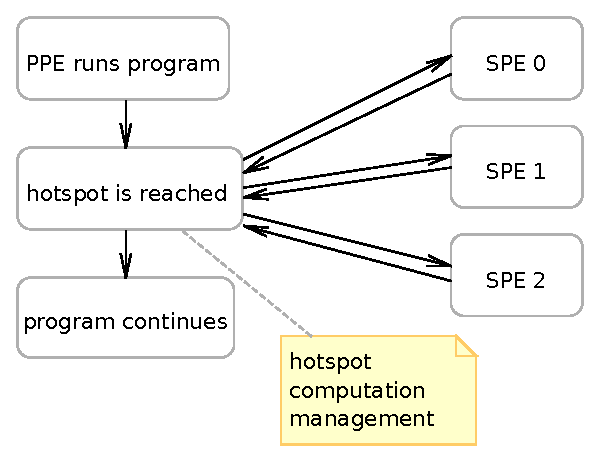
\includegraphics[width=0.7\textwidth]{data/PPUCentricModel}
    \caption[PPE centric configuration]{Program is run on PPE and only hotspots are offloaded to SPEs.
 Offloading means managing SPE context creation and loading as well as managing data transfer and synchronization between PPE and SPEs}
    \label{fg:PPUCentricModel}
\end{figure}

\item SPE server
\par
Another configuration is to have server-like programs running on SPEs that sits and waits offering specific services.
This is requires the code to be small enough to fit into the SPU local store along with processed data.

\end{enumerate}

\section {Building for the Cell/B.E.}
\par
Actual compilation process is performed using appropriate tool chain.
PPE code using of PPE tool chain and SPE code using SPE one.
But there is difference between management of code in linking stage between PPU and SPU object files.
It is caused by difference of actual code usage.
While PPU code resides in central memory, like in common architectures, SPU code is loaded into SPE dynamically and shall be somehow separated.
It is similar to shader programs for graphic accelerators.
They are also loaded into appropriate processors when they are needed so they live separated.

\par
There are two options for SPE code management.
One is to build shared library and load it explicitly when it is used.
Another way is to build a static library and include it into PPU executable using Cell/B.E. Embedded SPE Object Format (CESOF).
This allows PPE executable objects to contain SPE executable i.e. SPE binary is contained within PPE binary.
See figure \ref{fg:SPEEmbedding} how is SPE binary included into PPE binary.
This inclusion is called embedding and is performed with extra tool from tool chain.
The SPU program is then referenced as special external structure direct from PPU code, instead of performing shared libraries loading.
Both ways have advantages and disadvantages which are the same as shared vs. static library usage ones on other platforms.
Shared library means better modularity and possibility of code alternation without whole executable rebuilding.
On the other hand additional management of such library is necessary in contrast to static SPE code into PPE binary embedding.


\begin{figure}
    \centering
    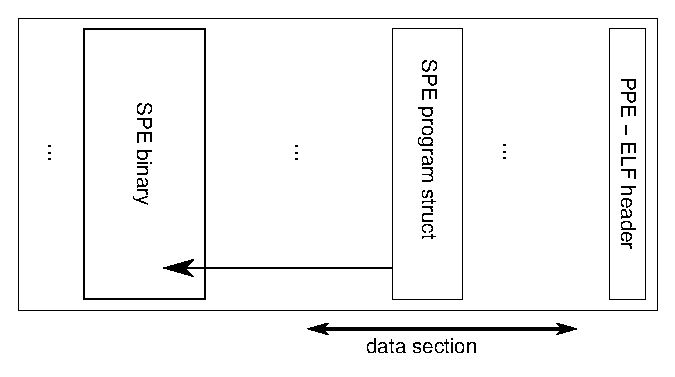
\includegraphics[width=0.8\textwidth]{data/SPEEmbedding}
    \caption[SPE binary embedding]{Illustration how is SPE binary "embedded" into a PPE binary.
An SPE binary is another section of the PPE binary.
It is reachable through extern struct variable, that contains a pointer to the SPE binary.}
    \label{fg:SPEEmbedding}
\end{figure}



\subsection {Process of application porting for the Cell/B.E.}
\label{sect:portingProcess}

Common process of porting an application for the Cell/B.E. processor (figure \ref{fg:appPorting}) consists of next few steps:
\begin{enumerate}
\item Hotspot localization
\par
Through profiling of the application on PPE we find most compute intensive parts, hotspots.
How to profile the application see chapter 5 of \cite{programmersGuide}.

\item Hotspots porting for SPE
\par
Hotspot code is then moved to the SPEs i.e. the code adaptation for SPE features shall be performed.
This means DMA transfers instead of direct memory access, appropriate data structures or other changes utilization.
Data movement tuning, e.g. using different data structures, can be then performed until satisfactory performance is obtained.
\end{enumerate}

\par
Following steps are necessary for application optimization and speed-up.
Application of these steps leads to utilization of all the SPU features such as whole register set utilization, dual-issuing of instructions, SIMD execution and DMA transfers.
More detail in \cite{writingPerfApps} part 4:
\\
\begin{enumerate}
\item{Multi-buffering}
\par
Data that resides within central memory and are processed by SPE should be copied onto local store buffer before actual computation.
When there are more of these buffers the program can take advantage from asynchronous DMA transfer and can process current buffer while the next data are transferred to another buffer.
Then the buffers are simply swapped and the SPU need not to wait until the transfer of next data is complete.
See figure in the paragraph named "Hiding data-access latencies" in \cite{compilerOptions} for illustration.

\item{Branch elimination}
\par
Branchless instruction chain is succession of instructions without any conditional jump.
In other words there is no decision where to continue performed within such succession.
Elimination of branches elongates branchless instruction chain.
In such a chain all data always go through the same instructions that makes possible to perform SIMDation.
There is variety branch elimination methods.
Good information resource provides \cite{cellPerformance}.
This step brings more advantage because branching is problem for every processor.
Branch elimination is probabbly the most complicated step of the porting process.

\item{SIMDation}
\par
Means rewriting scalar code into vectorized to be able to use SIMD instruction.
In this step the most performance gain could be achieved because of multiple data processing by one instruction.
Every single piece of data should go through the exactly same order of instructions in SIMDized code.
Therefore is necessary to have long branchless instruction chain.
The most important method is arrays of structure to structure of arrays conversion.
The figure in the paragraph called "SIMDizing" in \cite{compilerOptions} shall illustrate processing data with SIMD instruction.

\par
SIMDizing brings also avoidance of usage rotation instructions which are necessary to move unaligned data into preferred slot.
Preferred slot is beginning of a register e.g. for short int it is the first 16 bits.

\item{Loop unrolling}
\par
Loop body is the code inside curly brackets of the loop.
This code is executed repeatedly until the loop condition is valid.
Loop unrolling means putting more loop bodies serially into code.
This decrease loop count and elongate the loop body letting the compiler to make more optimizations.
Example:
\begin{verbatim}
for(uint32 i=0; i<32; i++)
{
    printf(".");
}
\end{verbatim}
become (by loop unrolling with factor 2)
\begin{verbatim}
for(uint32 i=0; i<16; i++)
{
    printf(".");
    printf(".");
}
\end{verbatim}
The compiler can do more optimizations e.g. better instruction scheduling and register utilization.

\item{Instruction scheduling}
\par
Proper reorganization of instructions can give us more performance in some cases.
This step is performed by the compiler but it is possible to rearrange instructions manually in assembly language.

\item{Branch hinting}
\par
Give the processor hint where the program is rather going to continue after future branch.
It is done through insertion of special instructions.
This step should be again accomplished by the compiler but is possible to use apropriate assembly language instruction directly within the code.
\end{enumerate}

\par
The whole process is repeated for every single hotspot.

\begin{figure}
    \centering
    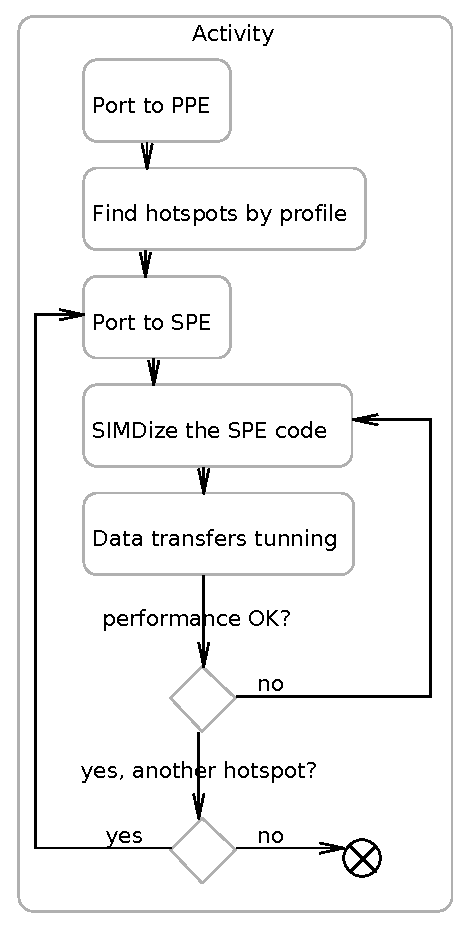
\includegraphics[width=0.5\textwidth]{data/portingCycle}
    \caption[Application porting cycle]{Diagram shows all stages of the process and loops for better performance tuning and other hotspots}
    \label{fg:appPorting}
\end{figure}

\subsection {SPE porting considerations}

\par
Local store size is the main SPE feature that everything spins around while porting code to SPE.
On the one hand are decisions about data transfers.
This means how the data that has to be processed by the SPE will be transferred into local store and vice versa.
What will be the sizes of data chunks.
How many buffers will be used in case of multi-buffering.
On the other hand is code complexity of the solved problem that influence the size of final binary.
There is one solution how to use bigger binaries than the local store, SPE overlays.
It is based on division of the binary into segments that are loaded into SPE on demand in run-time.

\par
Programmer has to take into consideration all these things to make the final binary smaller than local store.
Everything is big tradeoff between processed data chunk sizes with number of buffers of that chunks and code complexity i.e. how large algorithm can be.

\par
When compiling the SPU binary from ported code the final executable will probably increase the local store size even when the code seems not as large as the final binary size.
Then begins big searching what causes this huge size.
We have gone through several problems with code that is common in non SPE code but cause problems in SPE code.
Here is the list:
\begin{enumerate}
\item usage of keyword new
\par
There is no memory allocation on SPE. So new is meaningless.
But compiler accepts it without any complain.

\item usage of std streams
\par
This code:
\begin{verbatim}
#include <iostream>
std::cout << "Hello" << std::endl;
\end{verbatim}
goes through the compiler without complaints but makes the final binary too big.
The reason why the resulting code is too big is probably size of the code within headers that are included when using described features.

\end{enumerate}

\subsection {Speed and compiler options}

\par
There is variety of compiler options.
Usage of them is worth nothing but can increase performance and avoid some kind of bugs.

\par
Mike Acton explains in \cite{strictAliasing} the strict aliasing.
One advantage of usage of this option is its positive impact on performance.
Another advantage is fact that it can avoid bugs that would appear as far as in release stage when optimizations flags are used in compilation.
In this stage is this kind of bugs really hard to track and debug.

\par
Another option advises are in \cite{compilerOptions}

\section{Profiling}

\par
Profiling of Cell/B.E. application means rather profiling SPE part of the application.
There is variety of profiling tools.
The basic one is dynamic performance analysis which can provide many of useful information such as how much time the SPE stall and what reason, the CPI (cycle per instruction) ratio, branch count, etc.
The next one is static performance analysis which can illustrate run of SPE in instruction precision.
These two analysis are evaluated from program run within full system simulator.
Both the methods are well described in tutorial in the cell IDE help which is accessible through menu $\rightarrow$ Help $\rightarrow$ Help Content in IDE.

\par
Another profiling tools are:
\begin{enumerate}
\item{PDT - performance debugging tool}
\item{OProfile}
\item{CPC - cell performance counter}
\end{enumerate}

These tools collect profiling data that can be further processed with VPA (visual performance analyzer), external tool provided by IBM.
This tool can display the collected data in different charts, time lines or can highlight parts of code that are worth to improve and many other useful features.
Usage of all these performance tools is described in SDK document "Performance Tools Reference" in \cite{performanceToolRef}.
We wanted to test them all but when we follow the manual we experienced obstacles because we worked on PS3.
Lately, we found out on forums that unfortunately there is poor or none support for these performance tools on PS3.

\section{Segmentation}


\section{Level set algorithms}

formulace
urychlujici metody
segmentace pomoci levelsetu


Tabulka:::
\begin{center}
\begin{tabular}{|l|c|p{3.5in}|}
\hline
\multicolumn{3}{|c|}{Nazev tabulky}\\ 
\hline cell 1&cell 2&cell 3\\&todle bude pod cell 2, protoze to je mezi dvema'\&' &\\ 
\hline Big Basin&1.5&Very nice overnight to Berry Creek Falls from
either Headquarters or ocean side.\\ 
\hline Sunol&1&Technicolor green in the spring. Watch out for the cows.\\ 
\hline Henry Coe&1.5&Large wilderness nearby suitable for multi-day treks.\\ 
\hline
\end{tabular} 


\chapter{Tools setup}
\label{toolsSetup}

\section{SDK installation}

As first you have to do is to download actual SDK.
Go to \url{http://www-128.ibm.com/developerworks/power/cell/ downloads.html?S_TACT=105AGX16&S_CMP=LP}.
You should download following files:

\begin{enumerate}
\item SDK 3.1 Installer
cell-install-3.1.0-0.0.noarch.rpm  (11MB), contains install script and other stuff for SDK installation.
\item SDK 3.1 Developer package ISO image for Fedora 9
CellSDK-Devel-Fedora\_3.1.0.0.0.iso  (434MB), contains rpm packages that actual SDK is composed from (SDK packages)
\item SDK 3.1 Extras package ISO image for Fedora 9
CellSDK-Extras-Fedora\_3.1.0.0.0.iso  (34MB), contains some extra packages for Fedora
\end{enumerate}

Download it wherever you want (even though in documentation is /tmp/cellsdkiso).
Lets call the folder, you download it into, ISODIR.
First you shall stop the YUM updater daemon.

\begin{verbatim}
/etc/init.d/yum-updatesd stop
\end{verbatim}

If this outputs: bash: /etc/init.d/yum-updatesd: No such file or directory, you do not have any YUM updater daemon installed so you can skip this step.
Now issue following command to install required utilities for SDK installation

\begin{verbatim}
yum install rsync sed tcl wget
\end{verbatim}

Now install the downloaded installation rpm.

\begin{verbatim}
rpm -ivh ISODIR/cell-install-3.1.0-0.0.noarch.rpm
\end{verbatim}

After this step you have new stuff in /opt/cell installed. There is SDK installation script (cellsdk) located as well.
It is wrapper for YUM that manages the SDK packages. Run it with parameter --help to see the usage.
So next step is to run it.

\begin{verbatim}
/opt/cell/cellsdk --iso ISODIR -a install
\end{verbatim}

Parameter --iso tells to use downloaded ISOs and where can be found for mounting them onto loop-back device.
Parameter -a disables agreeing licenses. Otherwise you have to write some 'yes' to agree.
Process begins with setting local YUM repositories pointing to the ISOs.
Then all default packages are installed with all their dependencies.
To check result of the installation issue

\begin{verbatim}
/opt/cell/cellsdk verify
\end{verbatim}

Now we have SDK installed. Lets continue with installation of IDE.
It consists again of packages.
Now to simplify processing packages install yumex that provides graphical interface to YUM.
And lets you simply check packages that you want.

\begin{verbatim}
yum install yumex
\end{verbatim}

To install CellIDE run yumex, go to Group View$\rightarrow$Development$\rightarrow$Cell Development Tools.
Check \textit{cellide}, that is actual IDE (Eclipse with cell concerning stuff) and \textit{ibm-java2-i386-jre}, that is Java Runtime Environment, JRE needed for running of IDE.
And click 'Process Queue'. Note: you should have the ISOs mounted onto loop-back devices.
Otherwise you get 'Error Downloading Packages' after clicking 'Process Queue'.
So you have to mount ISOs whenever you want to install package concerning Cell SDK

\begin{verbatim}
/opt/cell/cellsdk --iso ISODIR mount
\end{verbatim}

After the installation you have two new folders.
/opt/cell/ide that contains the IDE and /opt/ibm/java2-i386-50 where JRE resides.
To run the ide you have to specify folder where the JRE is (through -vm param).

\begin{verbatim}
/opt/cell/ide/eclipse/eclipse -vm /opt/ibm/java2-i386-50/jre/bin/
\end{verbatim}

\section{IBM Full-System Simulator}

The last part of development environment is IBM Full-System Simulator (systemsim).
It is not part of ISOs with SDK so you have to download it separately.
Visit \url{http://www.alphaworks.ibm.com/tech/cellsystemsim/download} and download rpm with the simulator appropriate to the platform you are currently using.
Be sure to download fedora 9 version of the simulator (cell-3.1-8.f9.*). Then install it.

\begin{verbatim}
rpm -ivh ISODIR/systemsim-cell-3.1-8.f9.i386.rpm
\end{verbatim}

Maybe some dependencies will be missing. So you have to install it. In my case ot was libBLT24 and libtk8.5.

\begin{verbatim}
yum install blt tk
\end{verbatim}

Now you have simulator installed. But it has nothing to simulate.
Image with image of simulated Fedora 9 system is needed (sysroot image).
It is among SDK rpms so install it using yumex (Cell Development Tools$\rightarrow$sysroot\_image).
Now all necessary stuff is installed.
 You could start the IDE and start development. But there are some bugs to fix yet.

\subsection{Bug fixing}

If you start IDE and it crashes with unhandled exception it is probably caused by xulrunner library.
It is usually installed with Firefox3. There is following workaround:
\begin{enumerate}
\item download an older version of xulrunner

e.g. from: \url{http://releases.mozilla.org/pub/mozilla.org/xulrunner/ releases/1.8.1.3/contrib/linux-i686/ xulrunner-1.8.1.3.en-US.linux-i686-20080128.tar.gz}

\item untar to accessible directory

Lets call it XULDIR

\item edit the file

/opt/cell/ide/eclipse/eclipse.ini file as follows:
\label{XULLFIX}
\begin{verbatim}
...
-vmargs
-Dorg.eclipse.swt.browser.XULRunnerPath=XULDIR
...
\end{verbatim}
\end{enumerate}
Now you should start the IDE without the crash.

\par
Another issue (stack issue) is with tcl (scripting language that is used for configuration of the systemsim).
There is bug with stack size checking that causes cycling of tcl code.
To workaround this problem you should use ulimit command that changes default environment of Linux programs

\begin{verbatim}
ulimit -s unlimited
\end{verbatim}

causes that stack is unlimited.

\par
The last is to fix actual tcl script that manages loading the sysroot\_image (21\% issue - loading of the sysroot\_image freezes on 21\% so is not started and thats why unusable).
It is cause by wrong triggers that are triggerd when some text is output from console by the sysroot\_image loading.
There is probably triggers that wait for text from previous version of SDK that is never output in the current version.
That is why the loading freezes on 21\%.
To fix it you have to edit /opt/cell/ide/eclipse/plugins/ com.ibm.celldt.simulator.profile.default\_3.1.0.200809010950/ simulator\_init.tcl file.
Replace the "Welcome to Fedora Core" string with "Welcome to Fedora" and "INIT: Entering runlevel: 2" with "Starting login process".

It is useful to create starting script. That solve the stack issue and add systemsim directory to PATH (needed for running).

\begin{verbatim}
ulimit -s unlimited
PATH=/opt/ibm/systemsim-cell/bin:\$PATH
/opt/cell/ide/eclipse/eclipse -vm /opt/ibm/java2-i386-50/jre/bin
\end{verbatim}

\subsection{Installation of libraries into sysroot\_image}

Because sysroot\_image is provided as image of installed Fedora 9 without Cell B.E. libraries so next step is to install them into sysroot\_image.

\begin{verbatim}
/opt/cell/cellsdk_sync_simulator install
\end{verbatim}

This shell script installs all rpms for ppc and ppc64 platforms that finds in /tmp/cellsdk/rpms.
By default these rpms are copied into /tmp/cellsdk/rpms during the install process.
If they are not still there (or in installed subdirectory) you have to copy them by hand from ISOs (note: ISOs has to be mounted).

\begin{verbatim}
cp /opt/cell/yum-repos/CellSDK-Devel-Fedora/rpms/*.{ppc,ppc64}.rpm\
/tmp/cellsdk/rpms
\end{verbatim}

\subsection{Copying content into sysroot\_image}

Sysroot\_image is common binary image that can mounted and thus some additional content copied into.
This is useful when extra library that are not part of the default image need to be used.
In my case that was some boost libraries. So to mount the sysroot\_image issue:
\begin{verbatim}
mount -o loop /opt/ibm/systemsim-cell/images/cell/sysroot_disk <your mount point>
\end{verbatim}
And then copy whatever you want.

\subsection{Simulator hints}

\par
You can ssh to running simulator. It is better to use real bash that the console within IDE.
You have all the bash advantages like command and path completion available in contrast to 'text mode' of the IDE console.

\par
Sometimes root user is needed for an operation performed in the simulator.
Its password should be disabled.
It can be done when sysroot\_image is mouned.
Under host machine root account the sysroot\_image\_mount\_point/etc/passwd file should be edited.
The first line is the root's so deletion of '*' characted from the second field (after the second ':' character) will disable the root's password.
Note that this action must be performed when the simulator is not running otherwise the changes will be overwritten by the simulator.

\section{Setup CellIDE}

\section{Using examples}

Examples are installed into /opt/cell/sdk/src as tarball. So you have to untar each you want to use.
It is good to start with examples and tutorial sources.
Each folder has its own makefile that manages makefiles in its sub folders.
 So you can call only the top level one to build all projects in sub folders or any from the sub folders to build particular projects.

It is convenient to use the sample sources in CellIDE where you can build it as well and create run/debug configuration for running within cell environment.
To use the example code (for example /opt/cell/sdk/src/tutorial/simple) create new c++ makefile project.
Click right button on it to get into properties.
C/C++ general tab $\rightarrow$ Paths and Symbols $\rightarrow$ Source location.
Here you have to add the folder with the sources (/opt/cell/sdk/src/tutorial/simple) by 'create / link folder' button $\rightarrow$advanced $\rightarrow$ link to folder in filesystem.
Now you have two folders in list. The first one is the original, created during project creation and the other newly linked folder with the source.
You can delete the original one since you are not going to use it.
Next is necessary to set up 'Build directory' to tell the IDE where shall search for makefile.
It is C/C++ Build tab. Use 'Workspace' button to specify the folder because it will use workspace\_loc variable and thus independent on exact location on filesystem.

\section{Tuning memory usage on PS3}
\label{ps3MemoryUsage}

PS3 has only 256MB RAM memory. This is very small amount for operating system and programs together.
When install fedora system with default state and boot up it, the amount of remaining free memory is about 10MB.
It is insufficient for either debugging and compilation.
So some of resources has to be switched off.
Our PS3s are accessed remotely via ssh so there is no need for X server.
So this is the first you can turn off. This is performed by change of runlevel from 5 to 3.
Run level setting is in /etc/inittab file:
\begin{verbatim}
change in line "id:5:initdefault:" the 5 to 3
\end{verbatim}
Another resource are services.
Here you have to consider if the service you want to turn off is really unnecesary.
In Our PS3 NeworkManger and Wireless supplicant was turn off.
NOTE: when you turn off network manager, you have to turn on network service otherwise the networking will not run properly.
For service management within ssh console /usr/sbin/ntsysv manager is quite useful.
After disabling all unnecessary services we got about 130MB of free space.

Yellow dog distributions goes even beyond. They can access other 256MB in PS3 locked for graphics.
Special device is created and the graphic memory is the used as a swap partition. For details see \url{http://us.fixstars.com/products/ydl/}.

\section{Performance tools}

\begin{verbatim}
yum groupinfo "Cell Performance Tools"
\end{verbatim}

\section{Visual Performance Analyzer - VPA}

Another useful tool is VPA. It is not part of SDK so it should be downloaded separately.
Visit \url{http://www.alphaworks.ibm.com/tech/vpa} for details.
After installing (actually unpacking) the downloaded file similar fix in ini file to eclipse.ini file (see\ref{XULLFIX}) should be done to run the VPA correctly.

%--------------------------------------------------------
%-------------          REFERENCE           -------------
%--------------------------------------------------------

\bibliographystyle{plain}
\bibliography{references}

\end{document}